% !TEX program = xelatex
\documentclass[aspectratio=169]{beamer}

% Metropolis theme
\usetheme{metropolis}

% Packages
\usepackage{booktabs}
\usepackage{graphicx}
\usepackage{tikz}
\usetikzlibrary{shapes.geometric, arrows.meta, positioning}

% Custom colors (BFH corporate design inspired)
\definecolor{bfhblue}{HTML}{506e96}
\definecolor{bfhorange}{HTML}{fac300}

\setbeamercolor{frametitle}{bg=bfhblue}
\setbeamercolor{progress bar}{fg=bfhorange}

% Metadata
\title{INFFER Project: AI-Powered R Code Feedback}
\subtitle{A Scalable Learning Assistant for R Coding and Data Analytics}
\author{Ulrich Matter \& WDDA Team}
\institute{\textbf{Bern University of Applied Sciences (BFH)}\\[0.5em]
{\scriptsize\textit{Supported by BFH E-Learning funding program (virtuelle-akademie.ch)}}\\[0.2em]
{\scriptsize\textit{AI tools used: Claude Code (Sonnet 4.5, Opus 4.5) for app framework, testing, deployment, bug fixing, CSS styling, Beamer setup}}}
\date{December 15, 2025}

\begin{document}

% Title slide
\maketitle

% Slide 1: Motivation
\begin{frame}{The Challenge: Scaling R Coding Education}

\begin{columns}[T]
\begin{column}{0.55\textwidth}
\textbf{Teaching R coding at scale presents unique challenges:}
\begin{itemize}
    \item Students need \alert{immediate, personalized feedback}
    \item Instructors face high grading workloads
    \item Traditional office hours don't scale
    \item Students hesitate to ask ``basic'' questions
\end{itemize}

\vspace{1em}
\textbf{Our approach:}\\
Leverage large language models (LLMs) as on-demand tutoring assistants.
\end{column}

\begin{column}{0.4\textwidth}
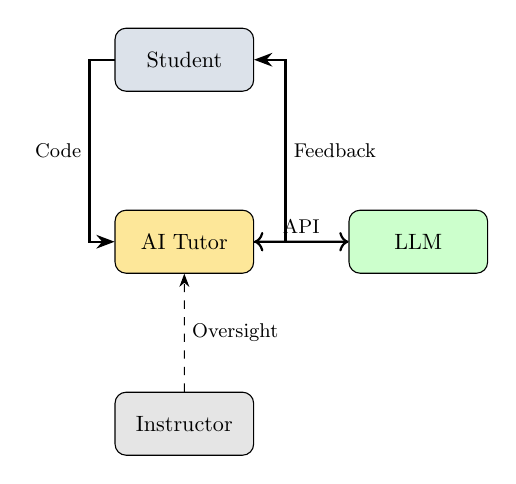
\begin{tikzpicture}[scale=0.8, every node/.style={scale=0.8}]
    \node[draw, rounded corners, fill=bfhblue!20, minimum width=2.2cm, minimum height=1cm] (student) {Student};
    \node[draw, rounded corners, fill=bfhorange!40, minimum width=2.2cm, minimum height=1cm, below=1.5cm of student] (ai) {AI Tutor};
    \node[draw, rounded corners, fill=gray!20, minimum width=2.2cm, minimum height=1cm, below=1.5cm of ai] (instructor) {Instructor};
    \node[draw, rounded corners, fill=green!20, minimum width=2.2cm, minimum height=1cm, right=1.2cm of ai] (llm) {LLM};

    \draw[-{Stealth}, thick] (student.west) -- ++(-0.4,0) |- node[left, font=\small, pos=0.25] {Code} (ai.west);
    \draw[-{Stealth}, thick] (ai.east) -- ++(0.5,0) |- node[right, font=\small, pos=0.25] {Feedback} (student.east);
    \draw[-{Stealth}, dashed] (instructor) -- node[right, font=\small] {Oversight} (ai);
    \draw[<->, thick] (ai) -- node[above, font=\small] {API} (llm);
\end{tikzpicture}
\end{column}
\end{columns}

\end{frame}

% Slide 2: Conceptual Background
\begin{frame}{Conceptual Background: AI in Education}

\textbf{Formative feedback} is critical for learning R coding:
\begin{itemize}
    \item Timely feedback improves learning outcomes (Hattie \& Timperley, 2007)
    \item Self-regulated learning requires actionable guidance
    \item Positive framing reduces anxiety and encourages experimentation
\end{itemize}

\vspace{1em}
\textbf{Why LLMs for code feedback?}

\begin{table}
\small
\begin{tabular}{lcc}
\toprule
\textbf{Capability} & \textbf{Traditional Tools} & \textbf{LLM-Based} \\
\midrule
Syntax checking & \checkmark & \checkmark \\
Unit tests / correctness & \checkmark & \checkmark \\
Style suggestions & Rule-based & Contextual \\
Conceptual explanations & Pre-written & Adaptive \\
Personalized tone & -- & \checkmark \\
Natural language interaction & -- & \checkmark \\
\bottomrule
\end{tabular}
\end{table}

\end{frame}

% Slide 3: Architecture (diagram only, large)
\begin{frame}{Architecture: Serverless \& Privacy-First}

\vspace{1cm}
\begin{center}
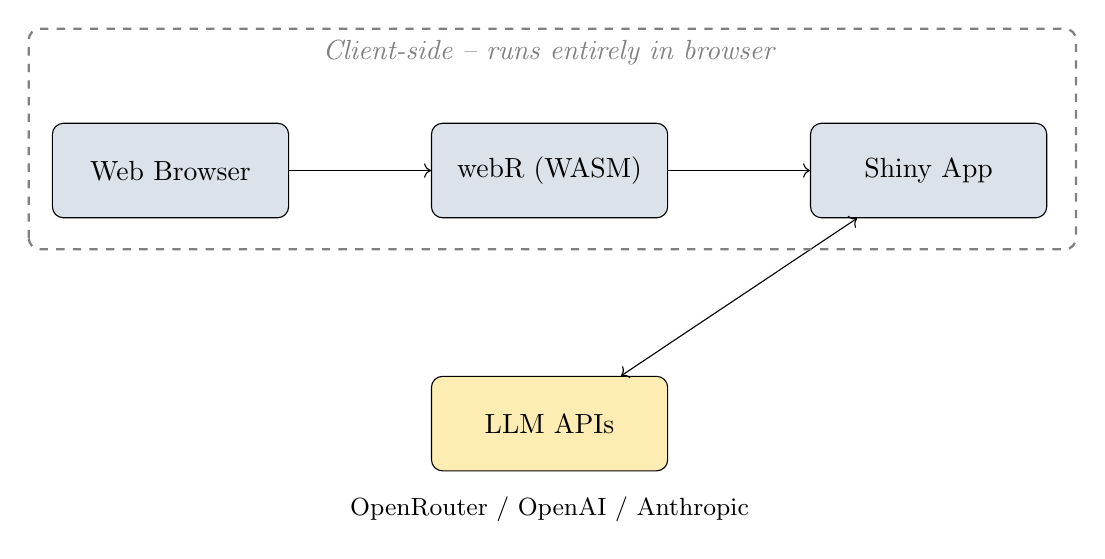
\begin{tikzpicture}[
    node distance=1.8cm,
    box/.style={draw, rounded corners, minimum width=3cm, minimum height=1.2cm, font=\normalsize},
    every edge/.style={draw, -{Stealth}, thick}
]
    % Browser layer
    \node[box, fill=bfhblue!20] (browser) {Web Browser};
    \node[box, fill=bfhblue!20, right=of browser] (webr) {webR (WASM)};
    \node[box, fill=bfhblue!20, right=of webr] (shiny) {Shiny App};

    % API layer
    \node[box, fill=bfhorange!30, below=2cm of webr] (api) {LLM APIs};
    \node[font=\small, below=0.2cm of api] {OpenRouter / OpenAI / Anthropic};

    % Arrows
    \draw[->] (browser) -- (webr);
    \draw[->] (webr) -- (shiny);
    \draw[<->] (shiny) -- (api);

    % Bounding box with label
    \draw[dashed, gray, rounded corners, thick] (-1.8, -1) rectangle (11.5, 1.8);
    \node[gray, font=\normalsize\itshape] at (4.8, 1.5) {Client-side -- runs entirely in browser};
\end{tikzpicture}
\end{center}

\end{frame}

% Slide 3b: Architecture - Key Design Principles
\begin{frame}{Architecture: Key Design Principles}

\begin{center}
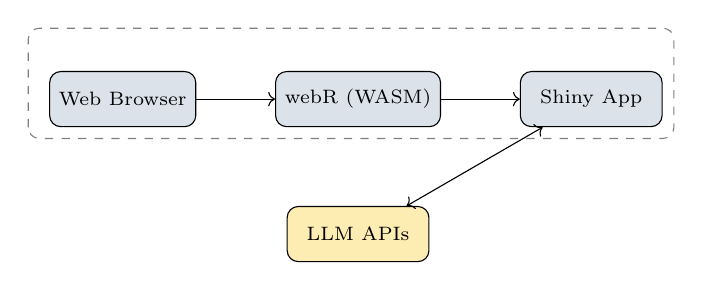
\begin{tikzpicture}[
    node distance=1cm,
    box/.style={draw, rounded corners, minimum width=1.8cm, minimum height=0.7cm, font=\scriptsize},
    every edge/.style={draw, -{Stealth}}
]
    % Browser layer (compact)
    \node[box, fill=bfhblue!20] (browser) {Web Browser};
    \node[box, fill=bfhblue!20, right=of browser] (webr) {webR (WASM)};
    \node[box, fill=bfhblue!20, right=of webr] (shiny) {Shiny App};

    % API layer
    \node[box, fill=bfhorange!30, below=1cm of webr] (api) {LLM APIs};

    % Arrows
    \draw[->] (browser) -- (webr);
    \draw[->] (webr) -- (shiny);
    \draw[<->] (shiny) -- (api);

    % Bounding box
    \draw[dashed, gray, rounded corners] (-1.2, -0.5) rectangle (7, 0.9);
\end{tikzpicture}
\end{center}

\vspace{0.8em}
\textbf{Key design principles:}
\begin{columns}[T]
\begin{column}{0.48\textwidth}
\begin{itemize}
    \item \textbf{Privacy by design}: No student code stored on any server
    \item \textbf{``Zero'' infrastructure}: Static hosting via GitHub Pages
\end{itemize}
\end{column}
\begin{column}{0.48\textwidth}
\begin{itemize}
    \item \alert{\textbf{BYOK model}}: Students use their own API keys (which we hand out)
    \item \textbf{Multi-provider}: Flexible model selection (via OpenRouter)
\end{itemize}
\end{column}
\end{columns}

\end{frame}

% Slide 4: Three-Layer Feedback System
\begin{frame}{Three-Layer Feedback System}

\begin{center}
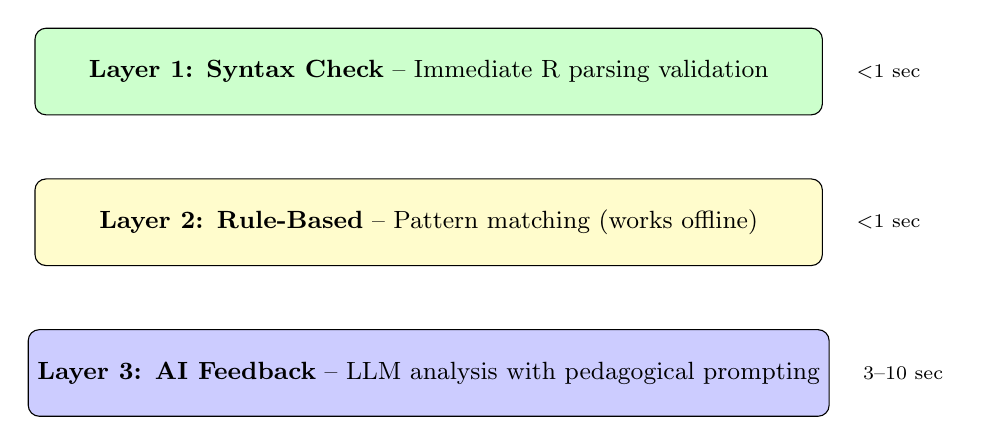
\begin{tikzpicture}[
    node distance=0.8cm,
    layer/.style={draw, rounded corners, minimum width=10cm, minimum height=1.1cm, font=\small},
]
    \node[layer, fill=green!20] (syntax) {
        \textbf{Layer 1: Syntax Check} -- Immediate R parsing validation
    };
    \node[layer, fill=yellow!20, below=of syntax] (rules) {
        \textbf{Layer 2: Rule-Based} -- Pattern matching (works offline)
    };
    \node[layer, fill=blue!20, below=of rules] (ai) {
        \textbf{Layer 3: AI Feedback} -- LLM analysis with pedagogical prompting
    };

    % Timing labels
    \node[right=0.3cm of syntax, font=\scriptsize] {$<$1 sec};
    \node[right=0.3cm of rules, font=\scriptsize] {$<$1 sec};
    \node[right=0.3cm of ai, font=\scriptsize] {3--10 sec};
\end{tikzpicture}
\end{center}

\vspace{0.5em}
\textbf{AI feedback is pedagogically prompted to:}
\begin{itemize}
    \item Start with positive observations
    \item Frame suggestions as learning opportunities
    \item Provide actionable next steps
    \item Use encouraging, supportive tone
\end{itemize}

\end{frame}

% Slide 5: Features & Intended Use
\begin{frame}{Features \& Intended Use}

\begin{columns}[T]
\begin{column}{0.48\textwidth}
\textbf{Key Features:}
\begin{itemize}
    \item Multi-language UI (EN/DE/FR)
    \item Screenshot paste support
    \item Configurable AI models
    \item Free tier options available
    \item Mobile-responsive design
\end{itemize}

\vspace{1em}
\textbf{Recommended Models:}
\begin{itemize}
    \item \alert{Qwen 2.5 Coder} -- Best for code
    \item DeepSeek V3 -- Best value
    \item Gemini Flash -- Free tier
\end{itemize}
\end{column}

\begin{column}{0.48\textwidth}
\textbf{Intended Use Cases:}
\begin{enumerate}
    \item \textbf{Self-study}: Students practice independently
    \item \textbf{Homework support}: Get unstuck without waiting
    \item \textbf{Exam prep}: Test understanding with instant feedback
    \item \textbf{Flipped classroom}: Pre-class coding exercises
\end{enumerate}

\vspace{1em}
\textbf{Not intended to replace instructor grading.}
\end{column}
\end{columns}

\end{frame}

% Slide 7: Demo Screenshot
\begin{frame}{Enjoy the Show}

\begin{center}
\includegraphics[width=0.85\textwidth,height=0.8\textheight,keepaspectratio]{app-screenshot.png}
\end{center}

\end{frame}

% Slide 8: Summary
\begin{frame}{Summary}

\textbf{What we built:}
\begin{itemize}
    \item AI-powered R code feedback tool
    \item Runs entirely in browser (no server)
    \item Privacy-preserving design
    \item Multi-model, multi-language support
\end{itemize}

\vspace{1.5em}
\textbf{Technology stack:}
\begin{itemize}
    \item R + Shiny + Shinylive
    \item webR (WebAssembly)
    \item OpenRouter / OpenAI / Anthropic APIs
\end{itemize}

\end{frame}

% Slide 9: Try it out & Questions
\begin{frame}{Try it out}

\begin{columns}[c]
\begin{column}{0.55\textwidth}
\begin{block}{}
\centering
\vspace{0.8em}
\textbf{Deployed at:}\\[0.3em]
\small{\url{https://umatter.github.io/inffer_feedback_app}}

\vspace{1em}
\textbf{Source code:}\\[0.3em]
\small{\url{https://github.com/umatter/inffer_feedback_app}}
\vspace{0.8em}
\end{block}
\end{column}

\begin{column}{0.4\textwidth}
\centering
\includegraphics[width=3.5cm]{qr-app.png}\\[0.3em]
{\footnotesize Scan to open app}
\end{column}
\end{columns}

\vspace{1em}
\centering
{\Large \textbf{Questions?}}

\end{frame}

\end{document}
